%!TEX root = ../template.tex
%%%%%%%%%%%%%%%%%%%%%%%%%%%%%%%%%%%%%%%%%%%%%%%%%%%%%%%%%%%%%%%%%%%%
%% chapter6.tex
%% NOVA thesis document file
%%
%% Chapter with lots of dummy text
%%%%%%%%%%%%%%%%%%%%%%%%%%%%%%%%%%%%%%%%%%%%%%%%%%%%%%%%%%%%%%%%%%%%

\typeout{NT FILE chapter6.tex}%

\chapter{Results and Discussion}
\label{cha:results}

\epigraph{
	In science, results are not the end, but the beginning of understanding.
}

\section{Performance of the RPC During the Experiment}

\subsection{RPC Acceptance}

An initial step in the analysis consisted in evaluating the performance of the \gls{RPC} during the experiment and compare it to expectations from the simulation campaign. This validation was necessary to ensure the reliability of subsequent analyses relying on \gls{RPC} data.

Figure \ref{fig:RPCHitMap} shows the hit map of the \gls{RPC} obtained from real experimental data alongside the corresponding map from the simulations. The comparison confirms that the \gls{RPC} acceptance during the experiment is consistent with the simulated expectations, providing confidence in the validity of the simulation framework for modeling \gls{RPC} response.

\begin{figure}
	\centering
	\begin{subfigure}{.43\textwidth}
		\centering
		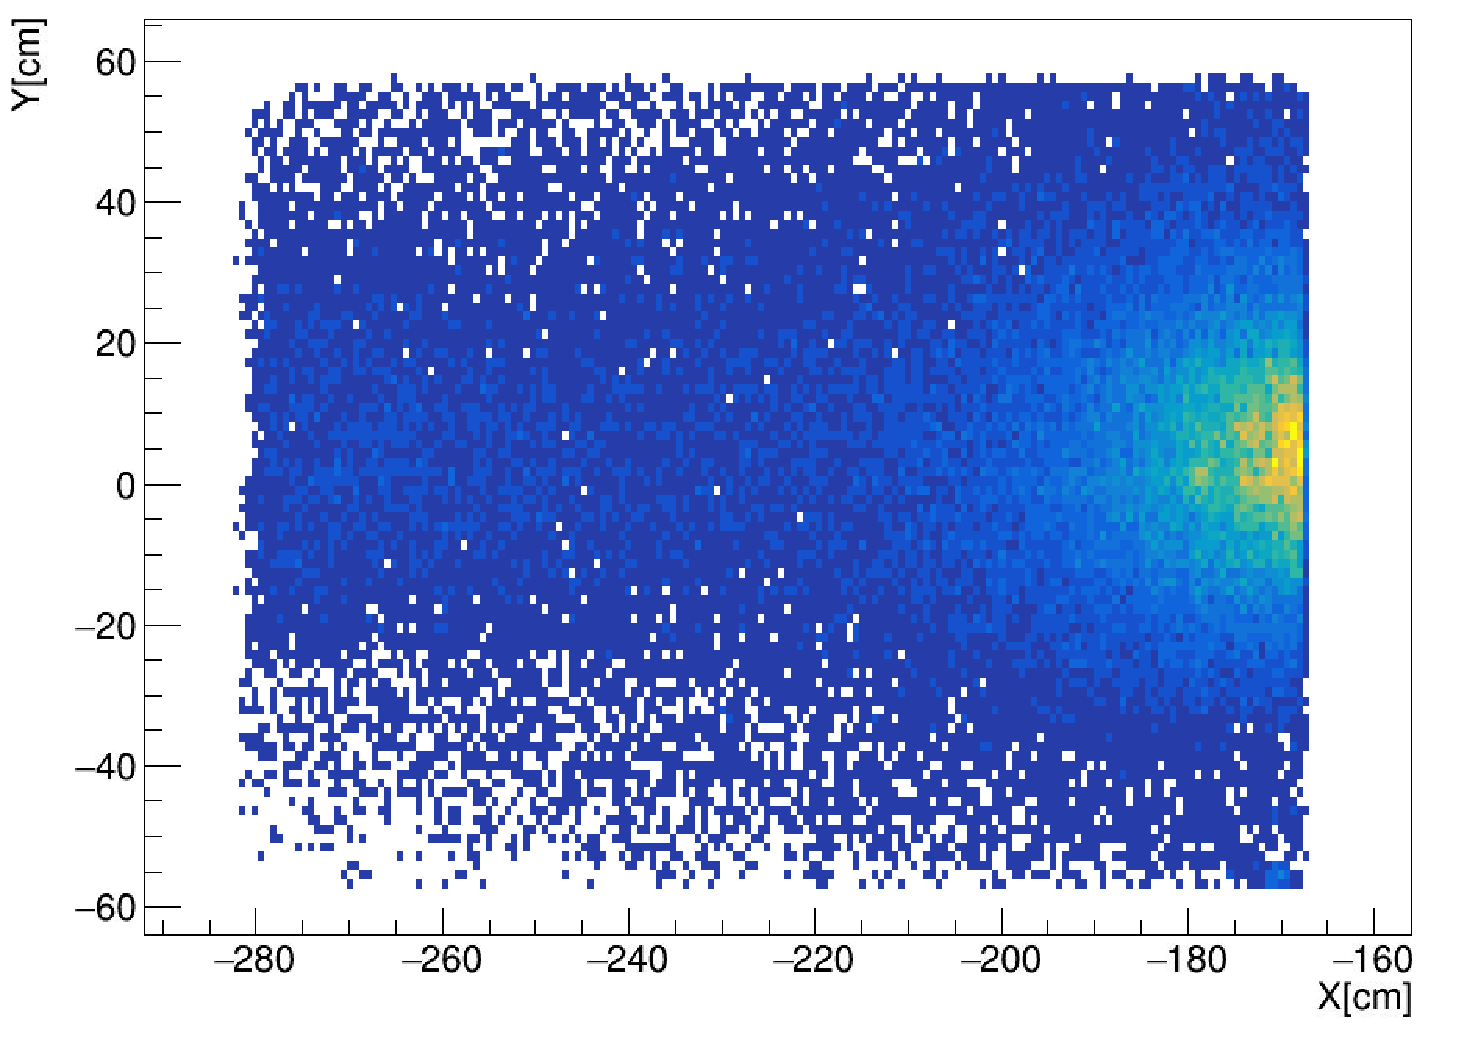
\includegraphics[width=\linewidth]{RealRPCHitMap}
		\caption{Experimental \gls{RPC} Hit Map}
		\label{fig:RealRPCHitMap}
	\end{subfigure}%
	\begin{subfigure}{.5\textwidth}
		\centering
		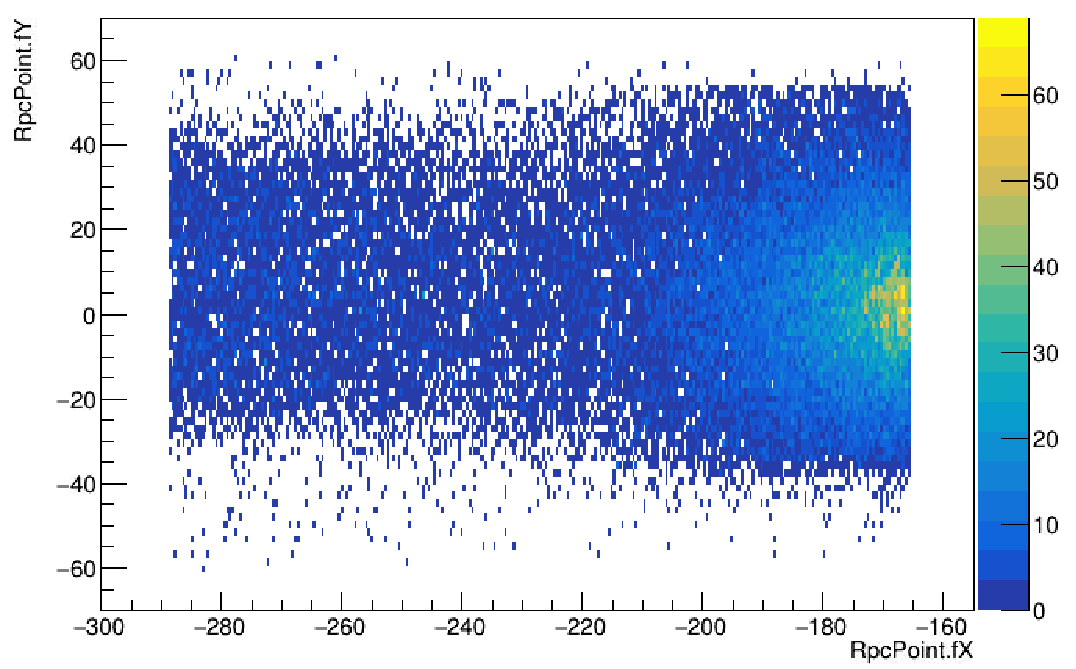
\includegraphics[width=\linewidth]{/Simulations/RPCSimHitMap}
		\caption{Simulated \gls{RPC} Hit Map}
		\label{fig:SimRPCHitMap}
	\end{subfigure}
	\caption[RPC hit map: experimental data vs. simulations]{Hit map of the \gls{RPC} obtained from experimental data compared to simulations. The consistency in the acceptance region validates the simulation framework for modeling \gls{RPC} response.}
	\label{fig:RPCHitMap}
\end{figure}

\subsection{Electronic Time Resolution}

To assess the electronic time resolution of the detector system, a dedicated pulser test was performed by simultaneously pulsing the LOS detector and the \gls{RPC} and measuring the time difference between the two signals. The resulting distribution, shown in Figure \ref{fig:RPCPulserTest}, yielded a Gaussian width of $\sigma = 38$~ps, which is in line with the performance observed in previous experiments and confirms the stability of the electronic chain.

\begin{figure}
	\centering
	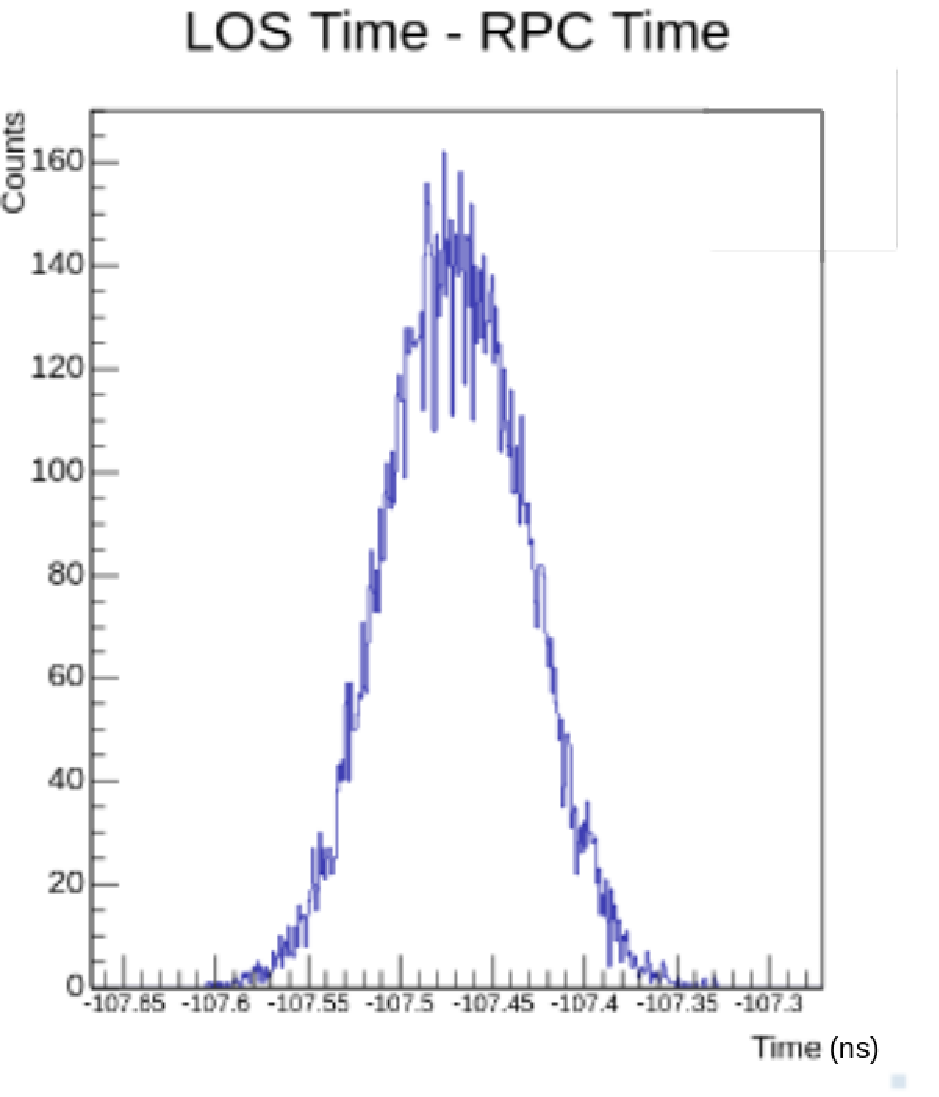
\includegraphics[width=0.5\linewidth]{RPCPulserTest}
	\caption[Time difference distribution between LOS and RPC signals]{Distribution of the time difference between LOS and \gls{RPC} signals obtained with a pulser test. The standard deviation of the distribution is $\sigma = 38$ ps, consistent with previous experimental results.}
	\label{fig:RPCPulserTest}
\end{figure}

\subsection{Time-of-Flight Calibration}

The time response of individual strips was further investigated by plotting the time-of-flight (ToF) as a function of the \gls{RPC} strip number (Figure \ref{fig:RPCToFCalibration}). While the majority of strips behaved as expected, several exhibited anomalous timing behavior, suggesting localized inefficiencies or calibration issues. This observation indicates that additional work will be required to properly account for these problematic strips, and it foreshadows challenges that will appear later in the analysis stage.

\begin{figure}
	\centering
	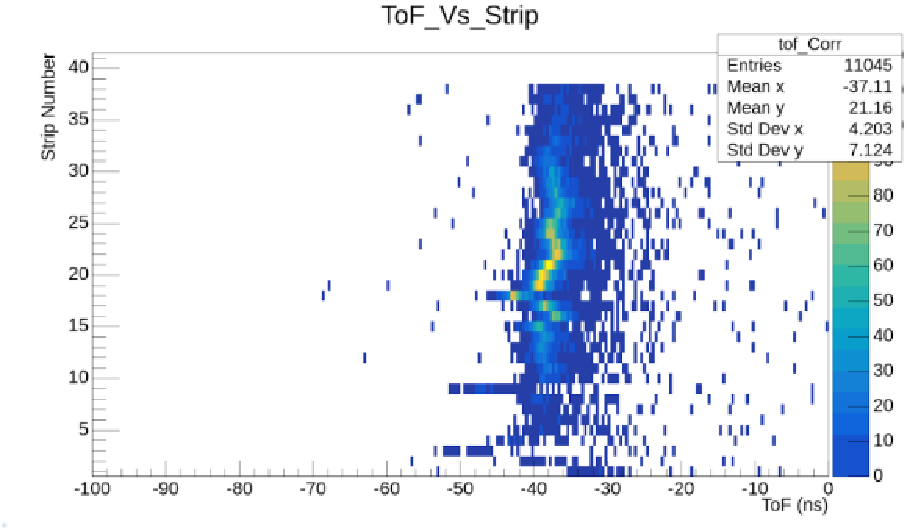
\includegraphics[width=0.8\linewidth]{RPCToFCalibration}
	\caption[Time-of-flight vs. RPC strip number]{Time-of-flight as a function of the \gls{RPC} strip number. Several strips show anomalous timing behavior, highlighting localized inefficiencies that require further calibration.}
	\label{fig:RPCToFCalibration}
\end{figure}

\subsection{Efficiency}

Finally, the overall efficiency of the \gls{RPC} was evaluated and is presented in Figure \ref{fig:RPCEfficiency}. The measured efficiency, of around 93\%, was found to be slightly below the levels achieved in previous experiments. This reduction can be attributed to the chosen operating conditions: while the nominal working point of the detector was 8250~V, during this experiment the high voltage applied to the resistive plates was deliberately set to 8000~V. This precautionary adjustment was taken to mitigate potential risks, given the lack of prior experience operating the \gls{RPC} with heavier fragments. Although it reduced the overall efficiency, this choice was necessary to ensure detector safety under the experimental conditions.

\begin{figure}
	\centering
	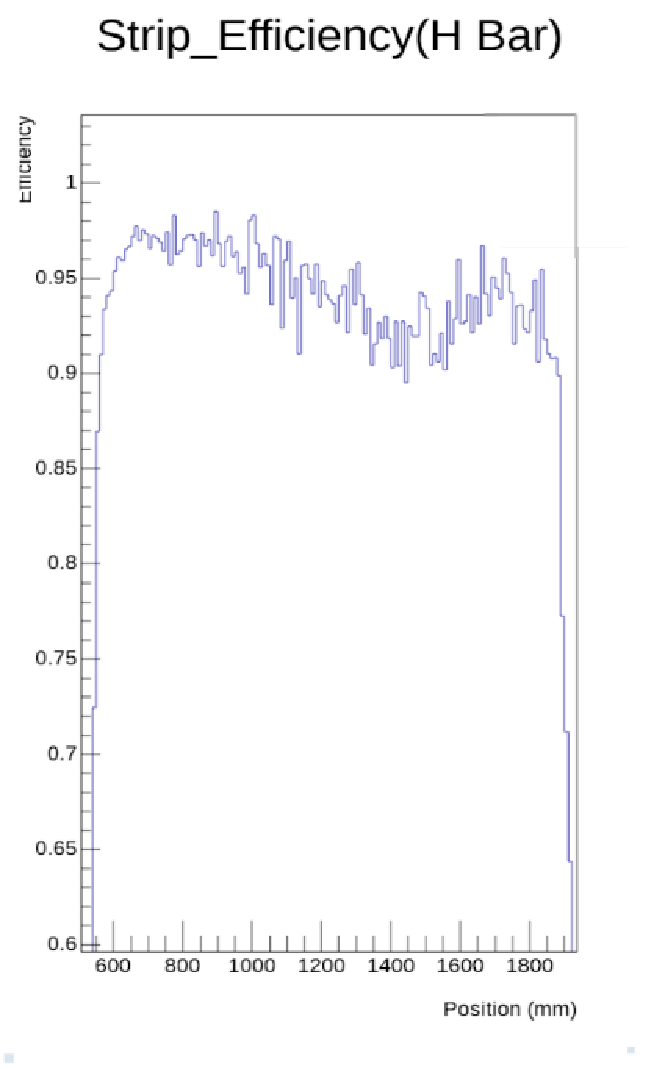
\includegraphics[width=0.5\linewidth]{RPCEfficiency}
	\caption[Overall RPC detection efficiency]{Overall \gls{RPC} detection efficiency. The slightly reduced performance compared to previous experiments is attributed to the lower operating voltage applied to protect the detector when exposed to heavier fragments.}
	\label{fig:RPCEfficiency}
\end{figure}



\section{MDF Method Application to Real Experimental Data}

After validating the \gls{MDF} models on simulated data, the next step was their application to real experimental events. To facilitate this analysis, an initial event selection strategy was implemented using the \gls{ToFD} detector as a veto. By requiring the absence of a \gls{ToFD} hit, it was possible to assume that the hits reconstructed in the FOOT detectors correspond directly to those reaching the \gls{RPC}, thus avoiding the ambiguities associated with multi-hit scenarios.

However, this approach introduces complications. A physical gap exists between the \gls{ToFD} and the \gls{RPC}, meaning that multi-fragment events can still occur where one fragment passes through the gap while another is detected in the \gls{RPC}. Additionally, charge determination using FOOTs alone is subject to limitations: at low charges, the FOOT resolution does not allow a clean separation between species with charges 2 and 3. Despite these caveats, the veto condition provides a practical starting point for the analysis.

To refine the selection and mitigate multi-hit ambiguities, an extended method was developed by explicitly including \gls{ToFD} information. When multiple FOOT hits are present, they are separated according to their reconstructed charges. The charge of the fragment reaching the \gls{RPC} is then inferred by comparing with the charge measured in \gls{ToFD}: if \gls{ToFD} registers a high charge, the lower-charge FOOT hit is selected for the \gls{RPC}, and vice versa. In cases where no \gls{ToFD} hit is present, the FOOT charge assignment is retained. Furthermore, when a \gls{ToFD} hit exists, the charge of the \gls{RPC} fragment is estimated as the difference between the incoming beam charge (given by LOS) and the \gls{ToFD} charge, assuming that the missing charge corresponds to the \gls{RPC} fragment. For the present analysis, events were selected with an incoming beam charge of 8 or 9 and with multiplicity one in the \gls{RPC}.

The results of applying the \gls{MDF} functions to real data show a mixed performance. The \gls{MDF} trained to reconstruct p/Q yielded consistent results, in agreement with expectations from simulations. This is evident from the comparison of the p/Q distributions in real and simulated data (Figure \ref{fig:PoQ_comparison}) as well as from the correlation between the \gls{RPC} hit position in the x-coordinate and the reconstructed p/Q, which follows the expected curve (Figure \ref{fig:x_vs_PoQ}). In contrast, the \gls{MDF} for A/Q did not perform as well. The reconstructed values exhibited a poor resolution and an unphysical tail toward zero, as shown in Figure \ref{fig:AoQ_hist}. In the particle identification (PID) plots of A/Q versus Q (Figure \ref{fig:PID_AoQ_vs_Q}), instead of well-separated blobs corresponding to different fragments, broad horizontal bands were observed due to the large dispersion in A/Q.

\begin{figure}
	\centering
	\begin{subfigure}{.57\textwidth}
		\centering
		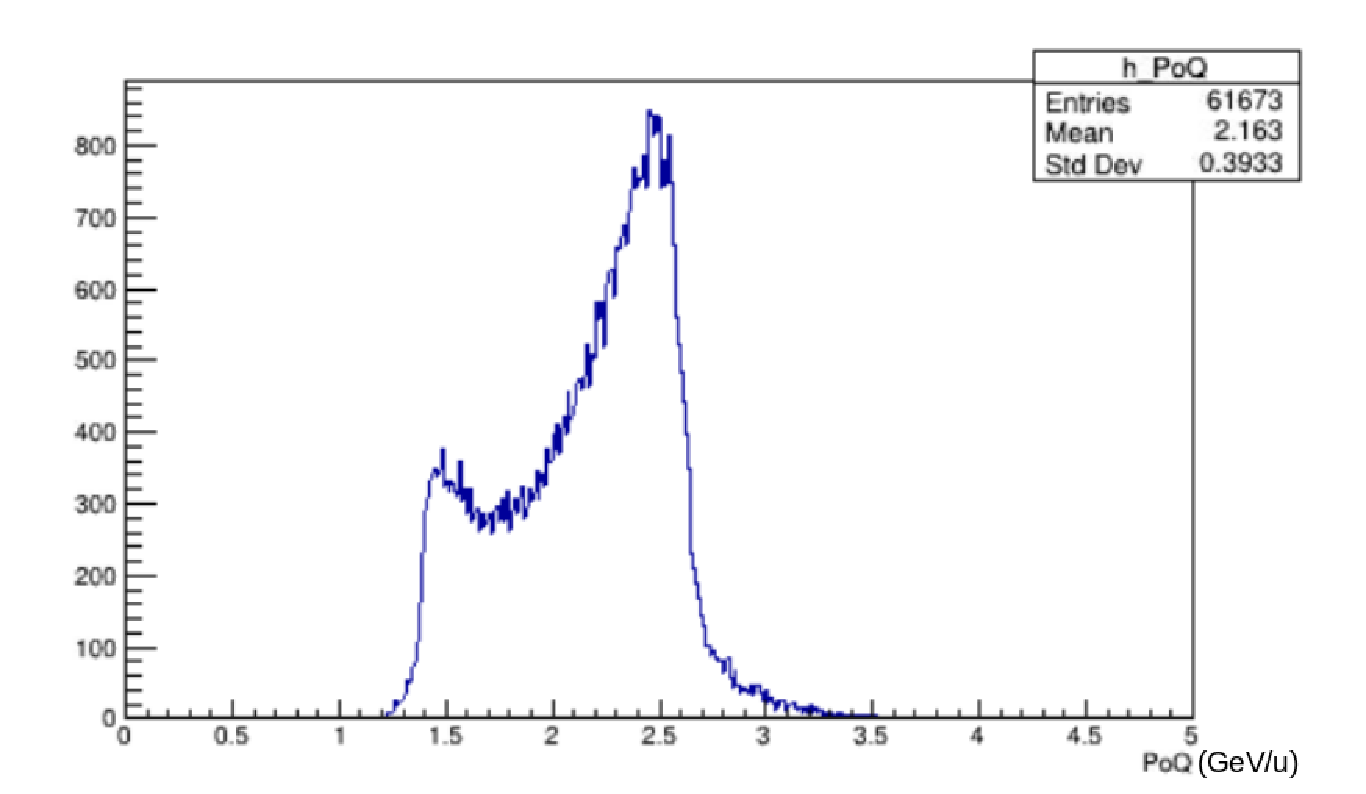
\includegraphics[width=\linewidth]{DataMDFPoQ}
		\caption{Real experimental data}
		\label{fig:DataMDFPoQ}
	\end{subfigure}%
	\begin{subfigure}{.43\textwidth}
		\centering
		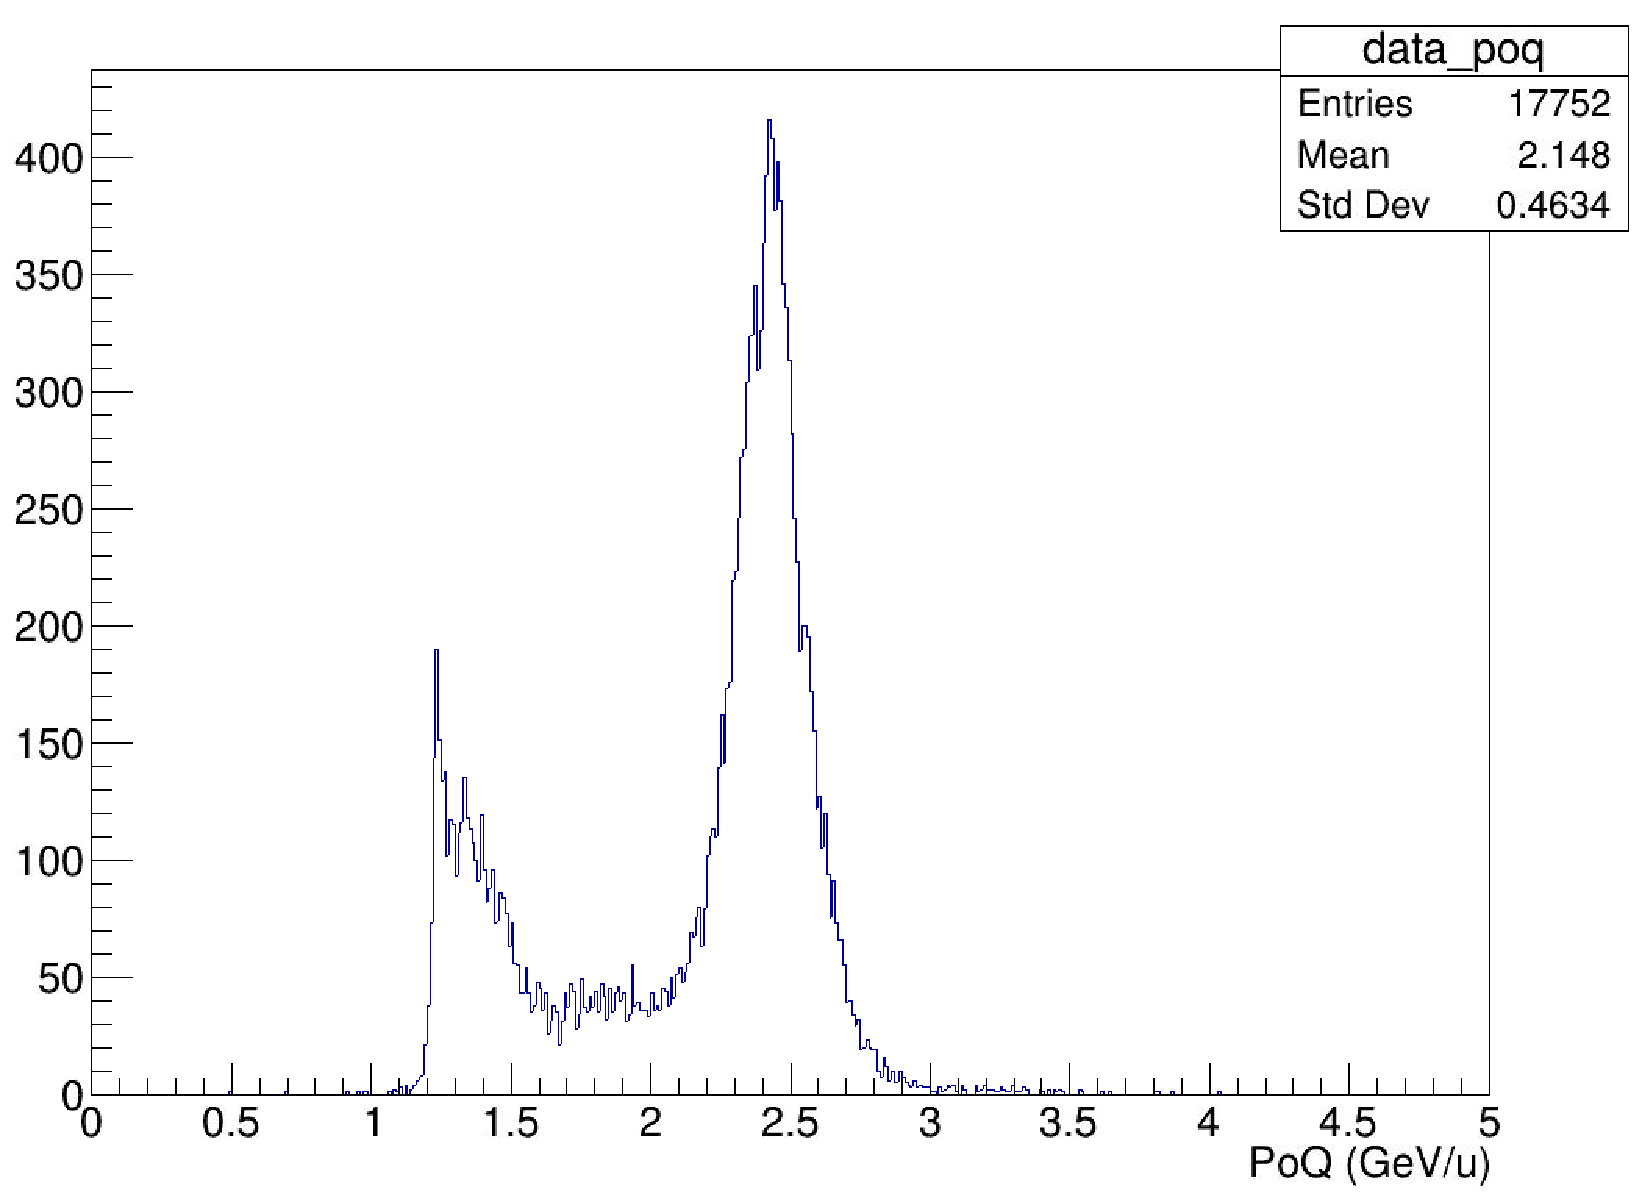
\includegraphics[width=\linewidth]{SimMDFPoQ}
		\caption{Simulated data}
		\label{fig:SimMDFPoQ}
	\end{subfigure}
	\caption[P/Q from MDF: experimental data vs. simulations]{Comparison of momentum-over-charge (p/Q) distributions reconstructed by the \gls{MDF}. The close agreement between both diagrams highlights the consistency of the \gls{MDF} performance across real and simulated conditions.}
	\label{fig:PoQ_comparison}
\end{figure}


\begin{figure}
	\centering
	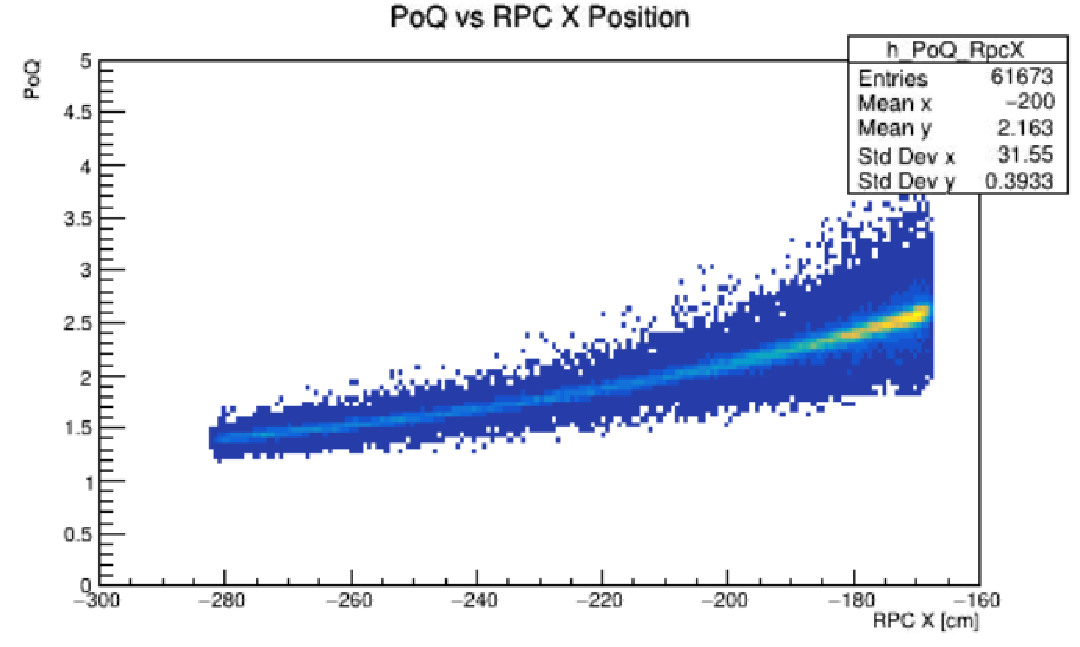
\includegraphics[width=0.7\linewidth]{DataMDFPoQvsX}
	\caption[RPC x-position vs p/Q]{Correlation between \gls{RPC} hit position in the x-coordinate and the reconstructed p/Q from real data. The expected curved dependence confirms the physical consistency of the \gls{MDF} results for p/Q.}
	\label{fig:x_vs_PoQ}
\end{figure}


\begin{figure}
	\centering
	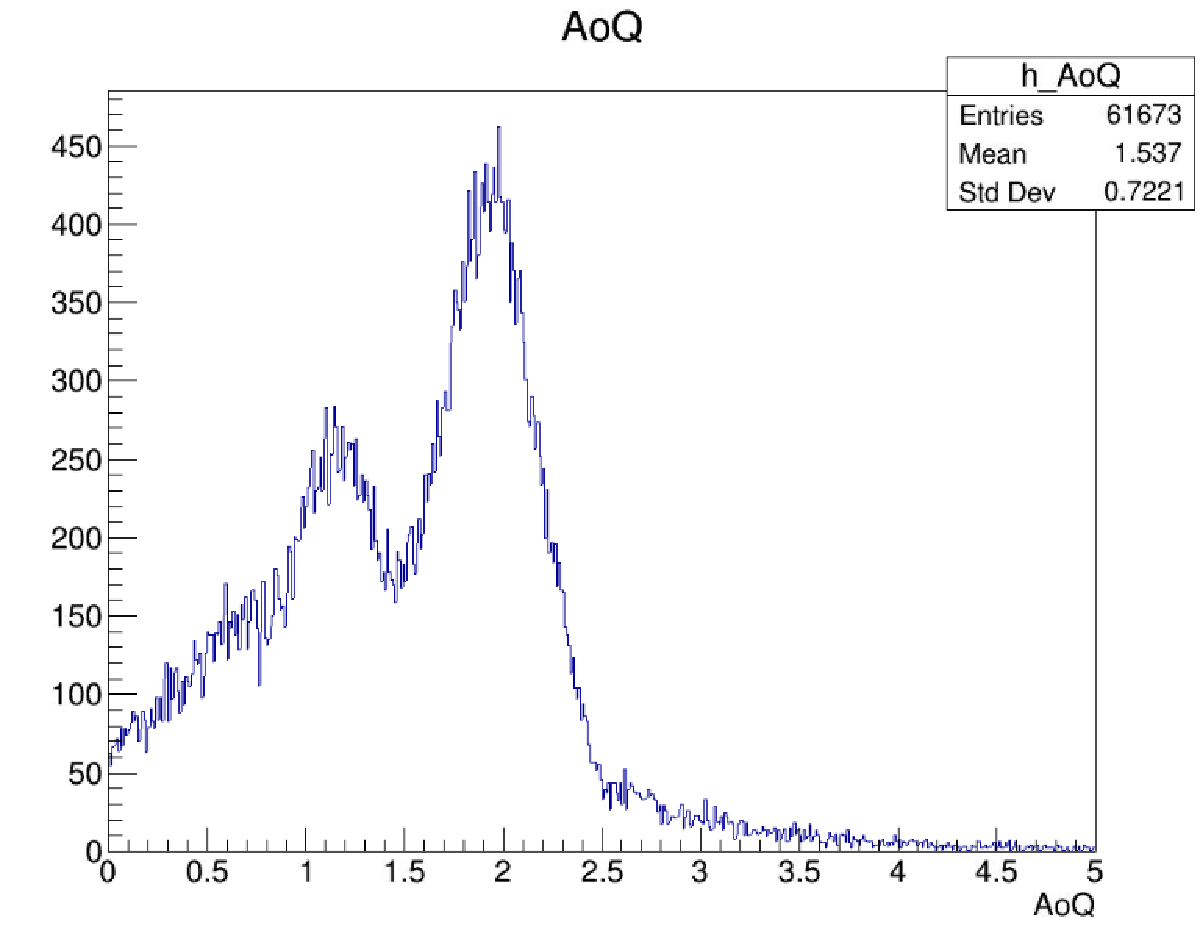
\includegraphics[width=0.7\linewidth]{DataMDFAoQ}
	\caption[Histogram of reconstructed A/Q]{Distribution of mass-to-charge ratio (A/Q) reconstructed by the \gls{MDF} from real experimental data. The broad dispersion and unphysical tail toward zero reflect the limitations of the current calibration stage.}
	\label{fig:AoQ_hist}
\end{figure}


\begin{figure}
	\centering
	\begin{subfigure}{.5\textwidth}
		\centering
		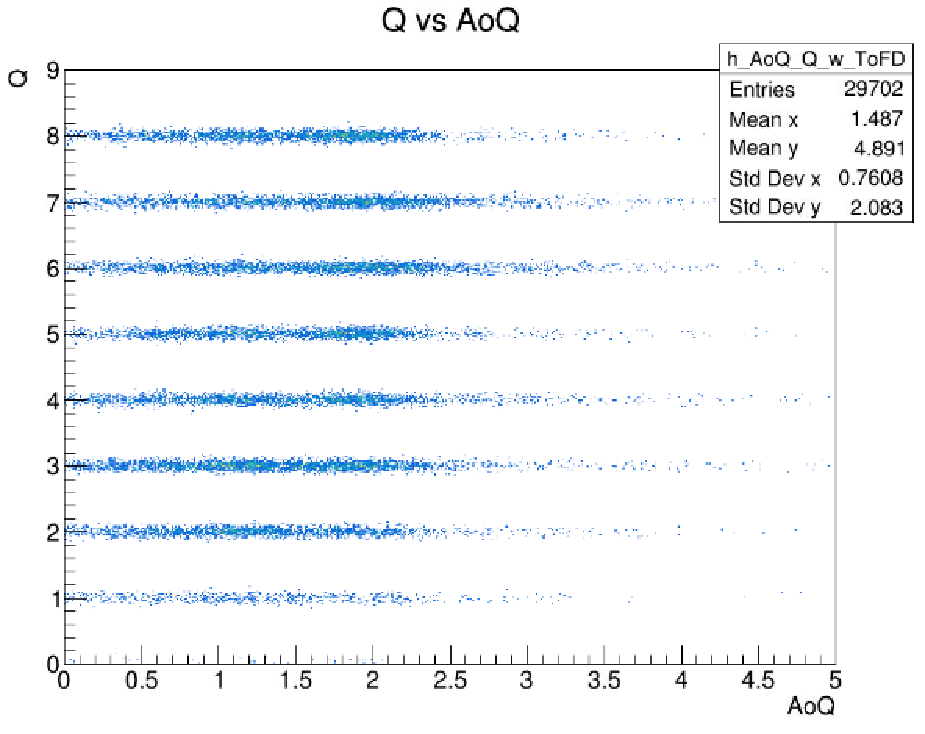
\includegraphics[width=\linewidth]{PIDwToFD}
		\caption{PID with \gls{ToFD}}
		\label{fig:PIDWToFD}
	\end{subfigure}%
	\begin{subfigure}{.5\textwidth}
		\centering
		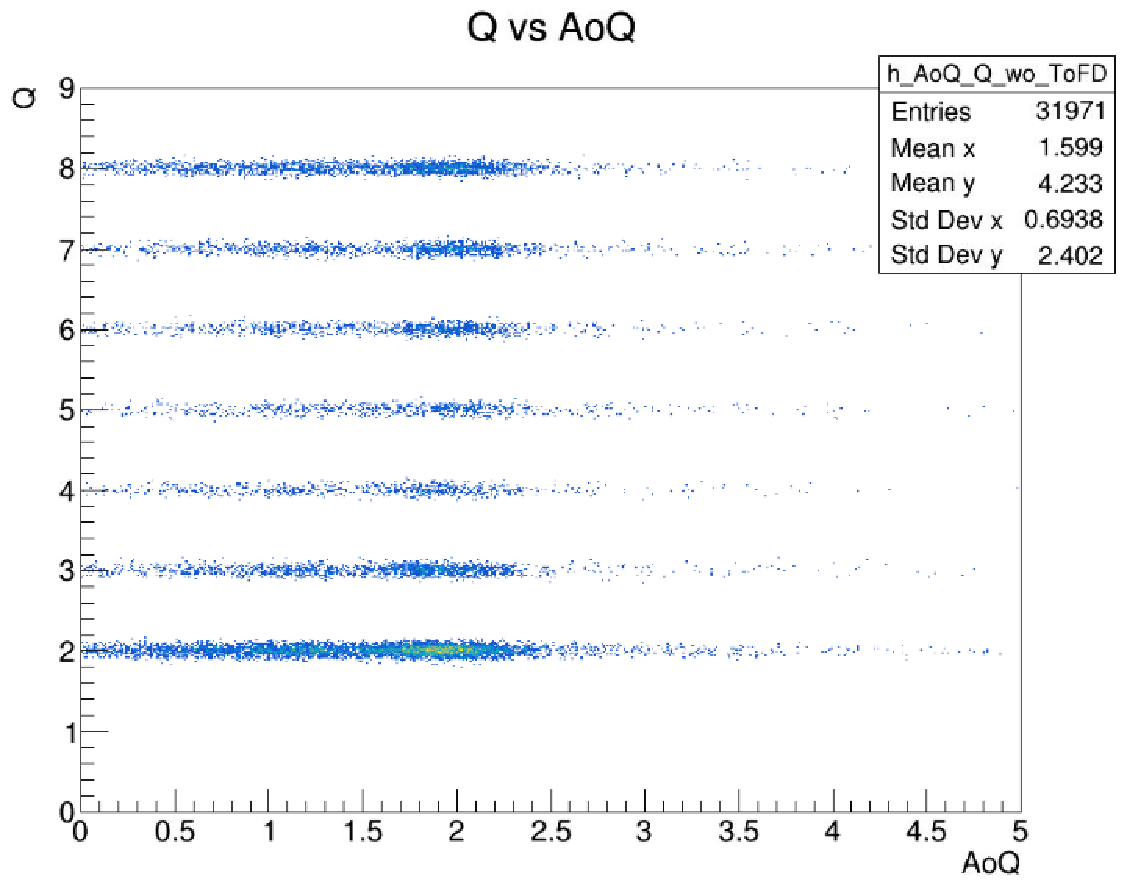
\includegraphics[width=\linewidth]{PIDwoToFD}
		\caption{PID without \gls{ToFD}}
		\label{fig:PIDwoToFD}
	\end{subfigure}
	\caption[PID plots (A/Q vs Q) with and without ToFD]{Particle identification plots of A/Q versus charge Q reconstructed by the \gls{MDF}. (a) Events selected with \gls{ToFD} information. (b) Events selected without \gls{ToFD} information. In both cases, instead of well-separated clusters, broad horizontal bands are observed, indicating poor A/Q resolution at this stage.}
	\label{fig:PID_AoQ_vs_Q}
\end{figure}

This behavior can be understood as a consequence of calibration limitations. At this stage, detector calibrations across the setup are still ongoing: while the \gls{RPC} calibration is being refined by the author, the FOOT detectors are under calibration by other members of the collaboration. From the simulation studies presented in Chapter \ref{cha:simulations}, it was shown that the \gls{MDF} prediction of A/Q is highly sensitive to the time-of-flight (TOF) observable. Indeed, by artificially worsening the TOF resolution in simulations, similar patterns emerge to those observed in real data, with highly dispersed A/Q values and horizontal PID bands. This strongly suggests that the current limitations originate from an incomplete calibration of the \gls{RPC} TOF response, as also evidenced earlier in the analysis of strip-dependent timing issues.

These findings highlight both the potential and the present challenges of applying \gls{MDF} to real experimental data. While the p/Q reconstruction is already promising, the reliable extraction of A/Q requires further improvements in detector calibration and possibly a more refined event selection strategy.


\section{Outlook and Future Work}

The present analysis should be regarded as preliminary. Future work will focus on completing the calibration of all relevant detectors, with particular emphasis on improving the \gls{RPC} time-of-flight determination. This step is expected to significantly enhance the \gls{MDF} performance for A/Q and enable clearer fragment separation in the PID plots. Additionally, further refinement of the hit selection procedure in the FOOT detectors and more stringent charge assignment strategies will be explored to reduce multi-hit ambiguities.

Ultimately, achieving robust PID reconstruction with the \gls{MDF} method would elevate the role of the \gls{RPC} beyond its traditional use as a proton and timing detector. It would position the \gls{RPC} as a versatile fragment detector, capable of contributing significantly to present \gls{R3B} experiments and future applications in the \gls{FAIR} High Energy Cave.


